\documentclass{beamer}
\usepackage[utf8]{inputenc}
\usepackage[frenchb]{babel}
\usepackage{lmodern}
\usepackage{amssymb}
\usepackage[T1]{fontenc}
\usepackage{listings}

\title{Oral du projet de Programmation Objet}
\author{Maxime Arthaud \and Martin Carton \and Korantin Auguste}

\date{13 mai 2013}

\begin{document}
  \begin{frame}
    \titlepage
  \end{frame}

  \begin{frame}{Introduction}
    Nous fournissons 3 choses:
    \begin{itemize}
      \item Un format de fichier pour pour pouvoir écrire des scènes à la main,
        dans une interface graphique ou automatiquement.

      \item
        Deux programmes:
        \begin{itemize}
          \item Une interface graphique pour éditer un fichier représentant une
            scène.
          \item Un programme en ligne de commande pour générer une image à
            partir d'un fichier de scène.
        \end{itemize}
    \end{itemize}
  \end{frame}

  \begin{frame}{Organisation}
    Nous avons découpé le travail:
    \begin{itemize}
      \item Maxime a principalement travaillé sur l'interface graphique.
      \item Martin a principalement travaillé sur le format de fichier,
        l'écriture d'images PPM et les classes représentant les objets.
      \item Korantin a principalement travaillé sur le lancer de rayon et les
        propriétés optiques.
    \end{itemize}
  \end{frame}

% ne pas indenter cette frame là, beamer et lstlisting interagissent mal
% ensemble
\begin{frame}[fragile]
\frametitle{Exemple de fichier}

\begin{lstlisting}
//exemple de scene :
Camera(eye=(0, 0, 0), origin=(-0.5, 0, 1.5),
       abscissa=(1, 0, 0), ordinate=(0, 1, 0),
       widthpixel=200, heightpixel=200)
AmbientLights(0.2, 0.2, 0.2)
Light(pos=(5, 0, 0), intensity=(0.5, 0.5, 0.5))
Sphere(center=(0, 5, 20), radius=3.14,
       k_diffuse=(0.6,0.3,0.6))
Plane(p1=(-1,0,30), p2=(1, 0, 30), p3=(0, 1, 30))
\end{lstlisting}
\end{frame}

  \begin{frame}{Interface utilisateur}
    \centerline{
      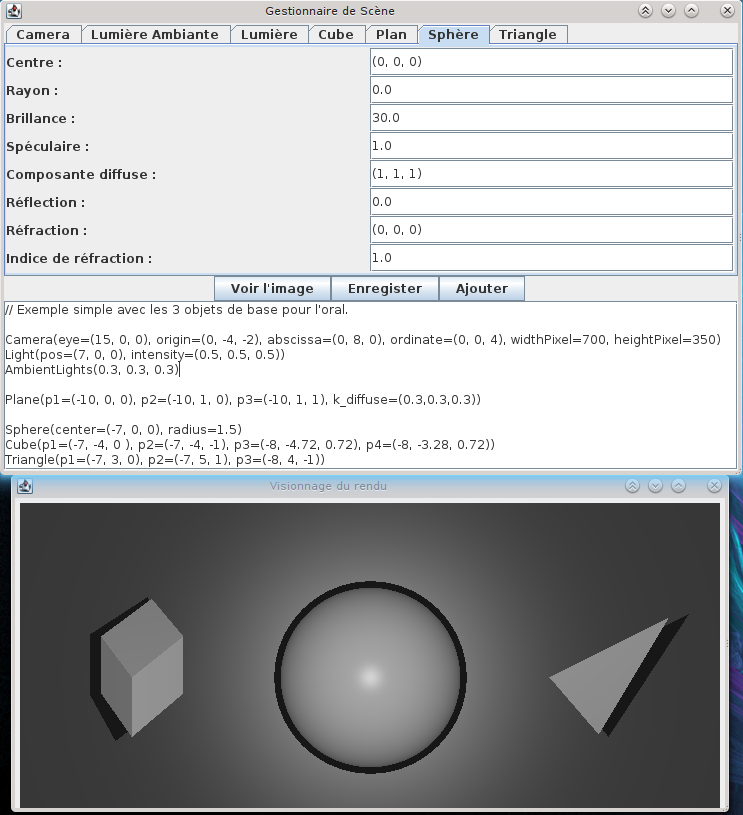
\includegraphics[height=0.8\paperheight, keepaspectratio=true]
      {screen2.png}
    }
  \end{frame}

  \begin{frame}{Conception de l'interface utilisateur}
      \centerline{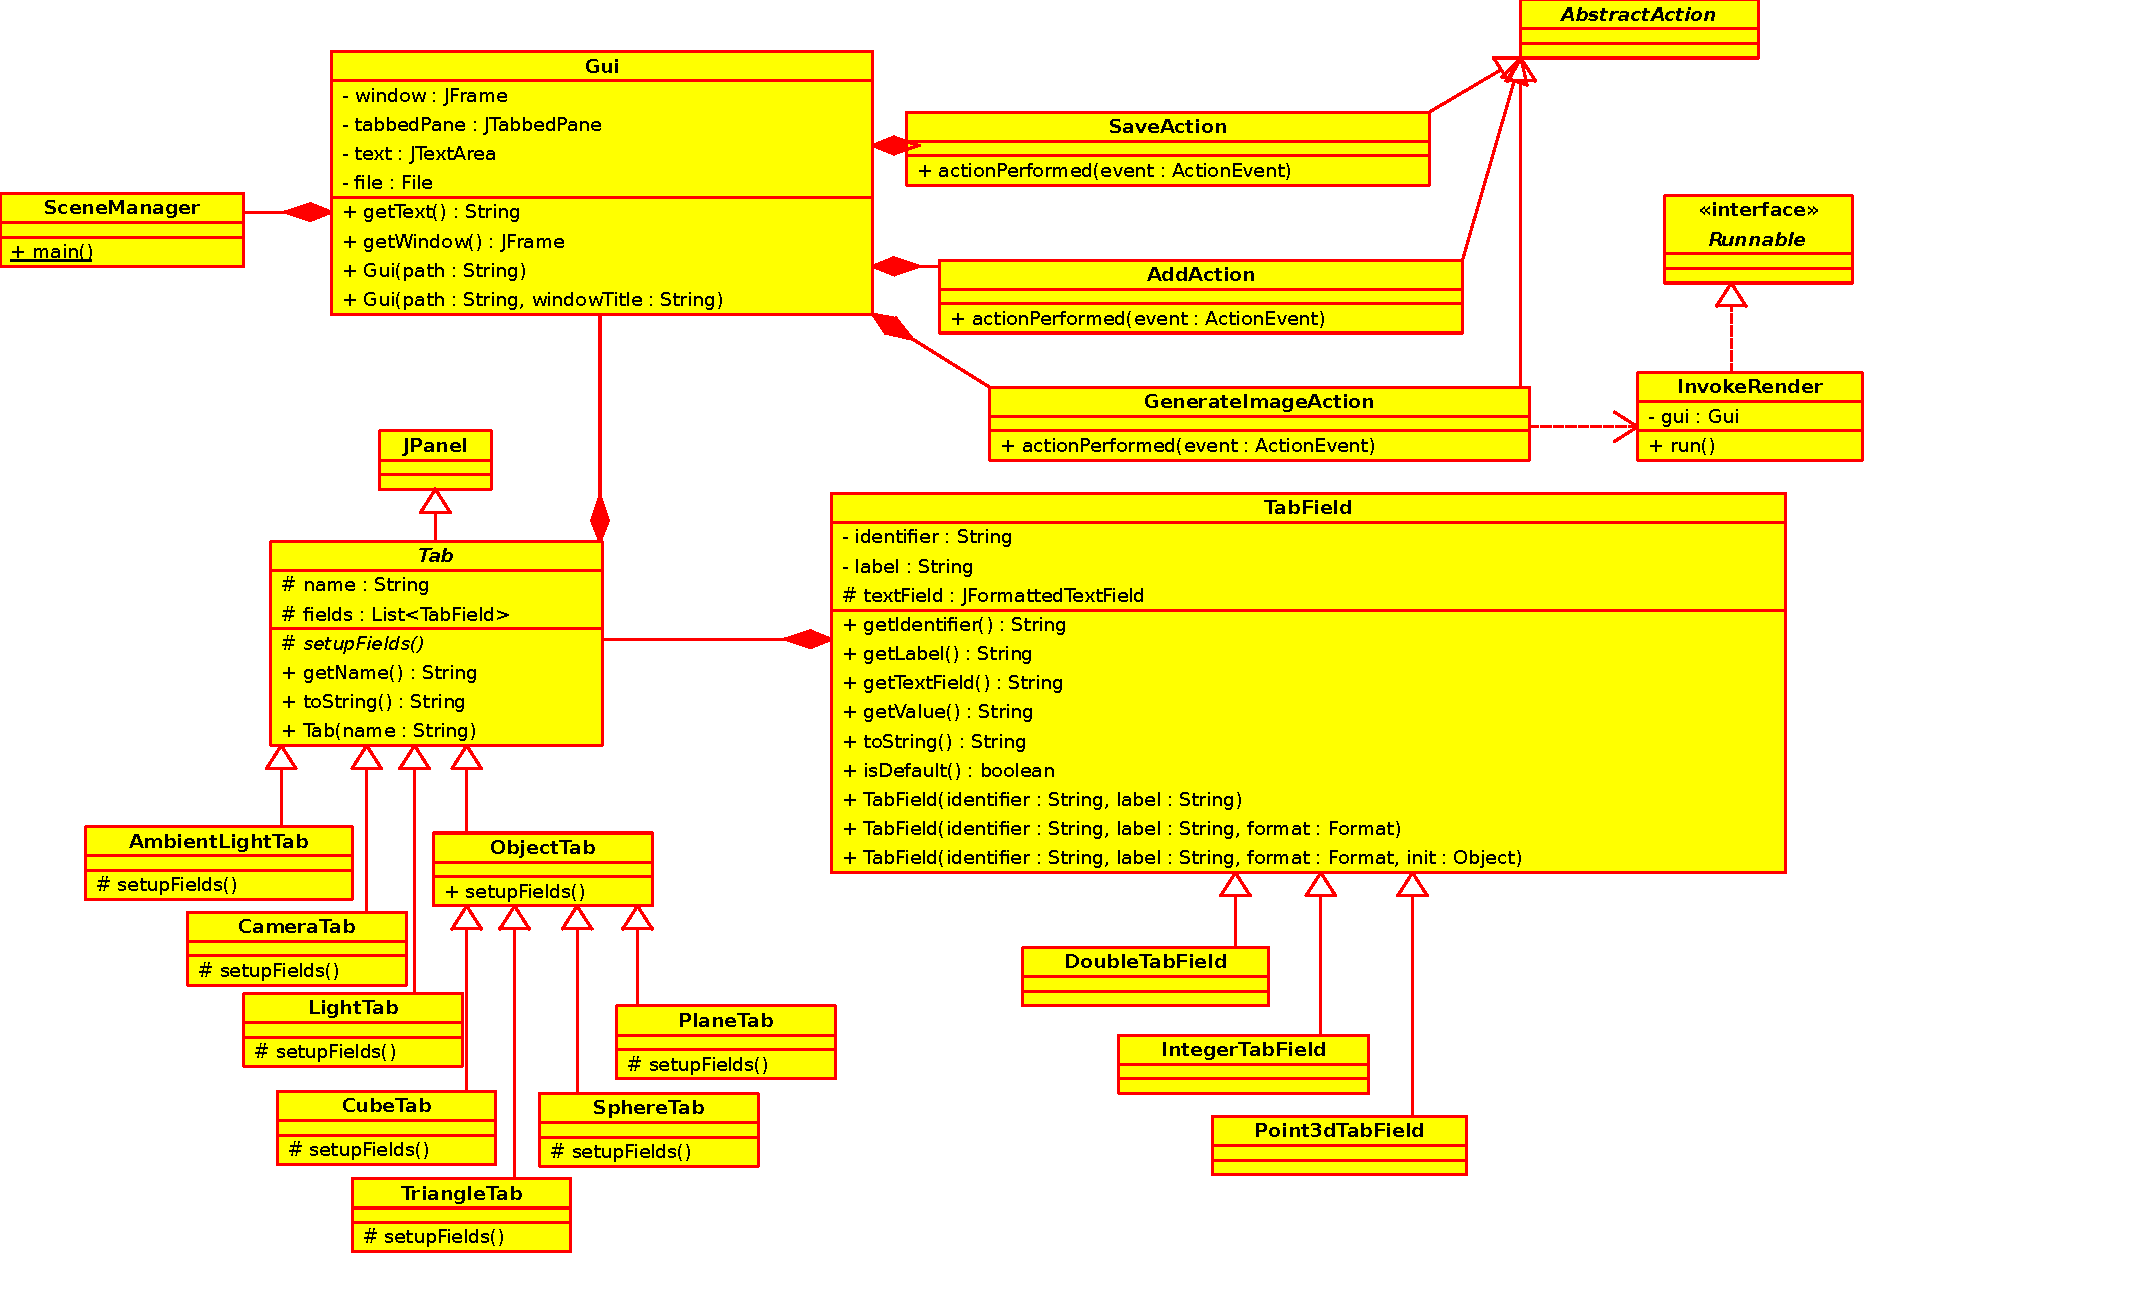
\includegraphics[width=0.95\paperwidth]{guiuml.pdf}}
  \end{frame}

  \begin{frame}{Conception du raytracer}
      \centerline{\includegraphics[width=0.95\paperwidth]{uml_hor.pdf}}
  \end{frame}

  \begin{frame}{Exemple de rendu plus complexe}
    \centerline{
      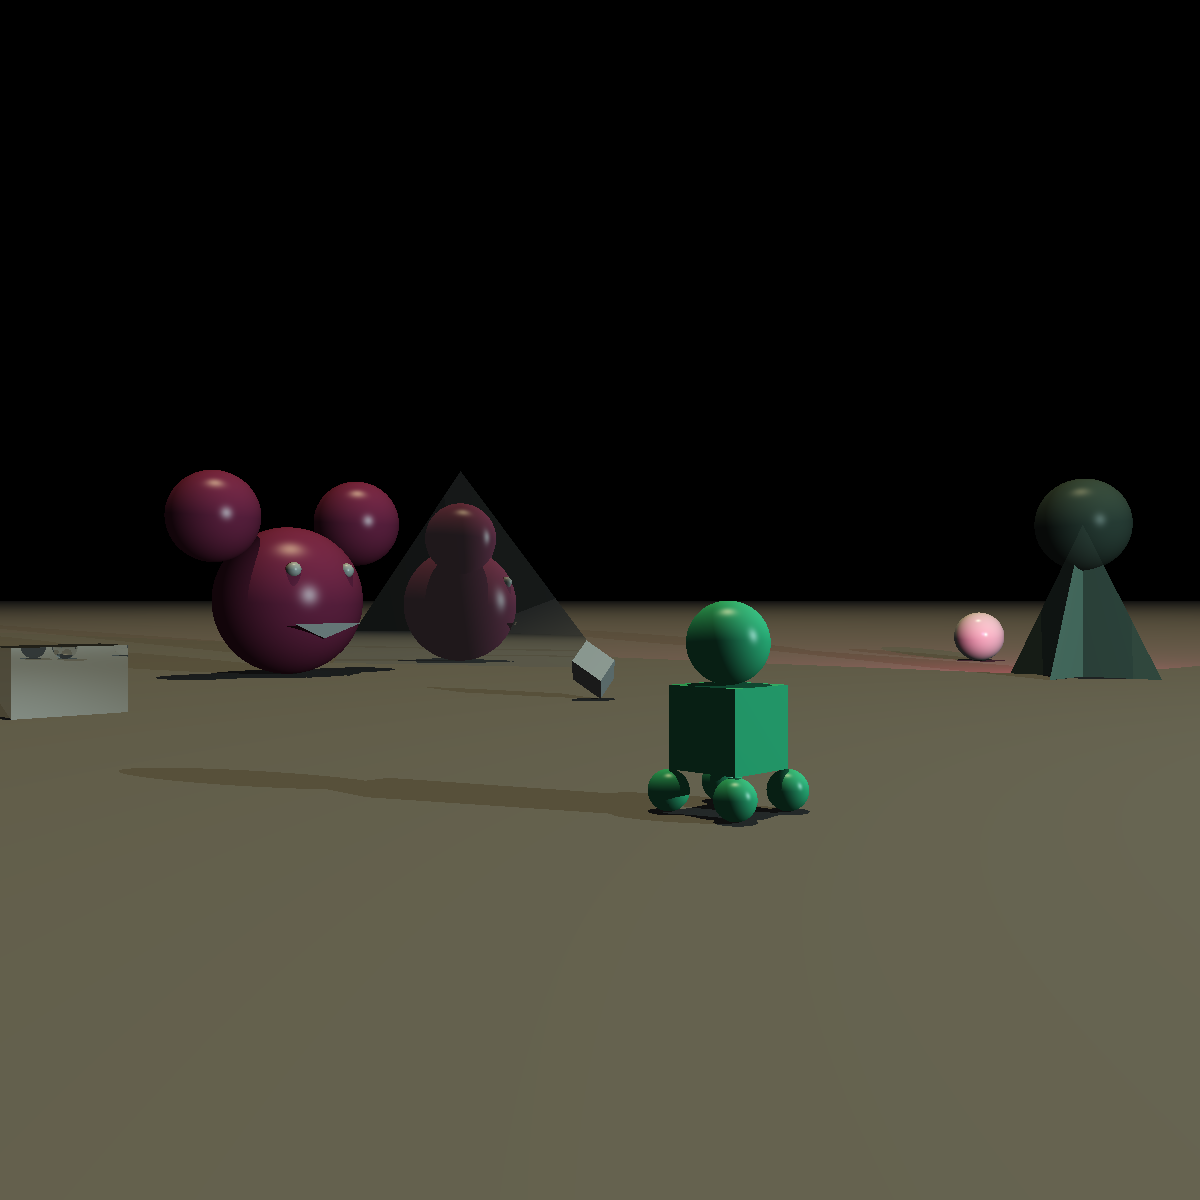
\includegraphics[width=\textwidth, height=0.8\paperheight,
      keepaspectratio=true]{0377.png}
    }
  \end{frame}

  \begin{frame}{Exemple de rendu plus complexe, autre point de vue}
    \centerline{
      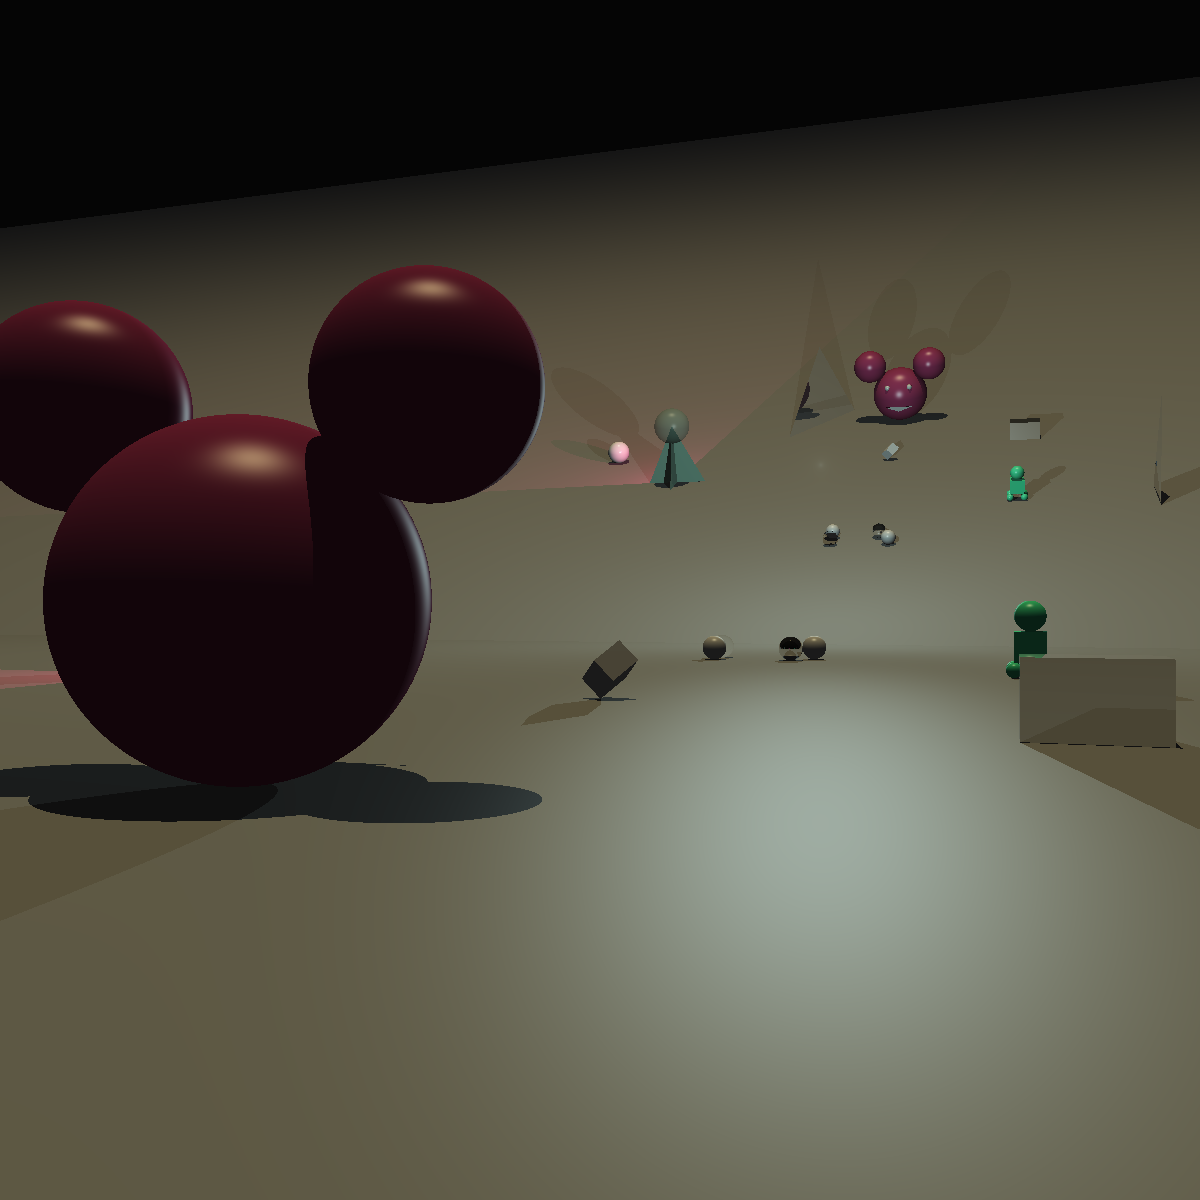
\includegraphics[width=\textwidth, height=0.8\paperheight,
      keepaspectratio=true]{0699.png}
    }
  \end{frame}

  \begin{frame}{Problèmes rencontrés}
    \begin{itemize}
      \item Un objet peut s'intersecter avec lui-même.
      \item La réfraction, notamment dans une sphère, n'est pas très réaliste.
      \item Complexité en $O(x\times y\times n^2 \times m)$ avec $n$ le nombre
        d'objets et $m$ le nombre de sources lumineuses.
    \end{itemize}
  \end{frame}

  \begin{frame}{Améliorations}
    \begin{itemize}
      \item Support de plusieurs formats de fichier.
      \item Possibilité de mettre une image sur un Parallélogramme.
      \item Création de vidéos.
    \end{itemize}
  \end{frame}
\end{document}

